\chapter{Proposed System}

In this section the full sensor setup is described step by step and design choices are justified. In the first part the concept of different modes are presented.



\section{Operating Modes}

In order to measure the information carrying signals, respectively the resistor values as described in section \ref{sec:3port}, the voltage supply on the pins has to be switched. The resistor values can be then used to detect position. Mode 1 in fig. \ref{fig:operatingmode} shows the arrangement how the voltage drop over R\textsubscript{1} is measured by the voltage divider in equation \ref{eq:divider}. For the following equation the terminology R(F) is used, where "F" refers to force dependency. Therefore as mentioned already in chapter \ref{ch:overview} the FSR is no true force sensor due to the area dependency.\newline
An alternative solution to the system presented here would be to have load resistances at the pins connected to R\textsubscript{1} and R\textsubscript{2}. The only difference would be that e.g. in the first mode when no force is applied the signal would be zero instead of the supply voltage as it is in the presented arrangement. Then if force was applied signal would rise instead of drop. However, as already mentioned in \ref{subsection:setup} it would not make any difference for the measurements. For this method an additional resistor and an additional pin on the PSoC would have been needed and therefore the initial presented method was used.

\begin{figure}[htp]
    \centering
    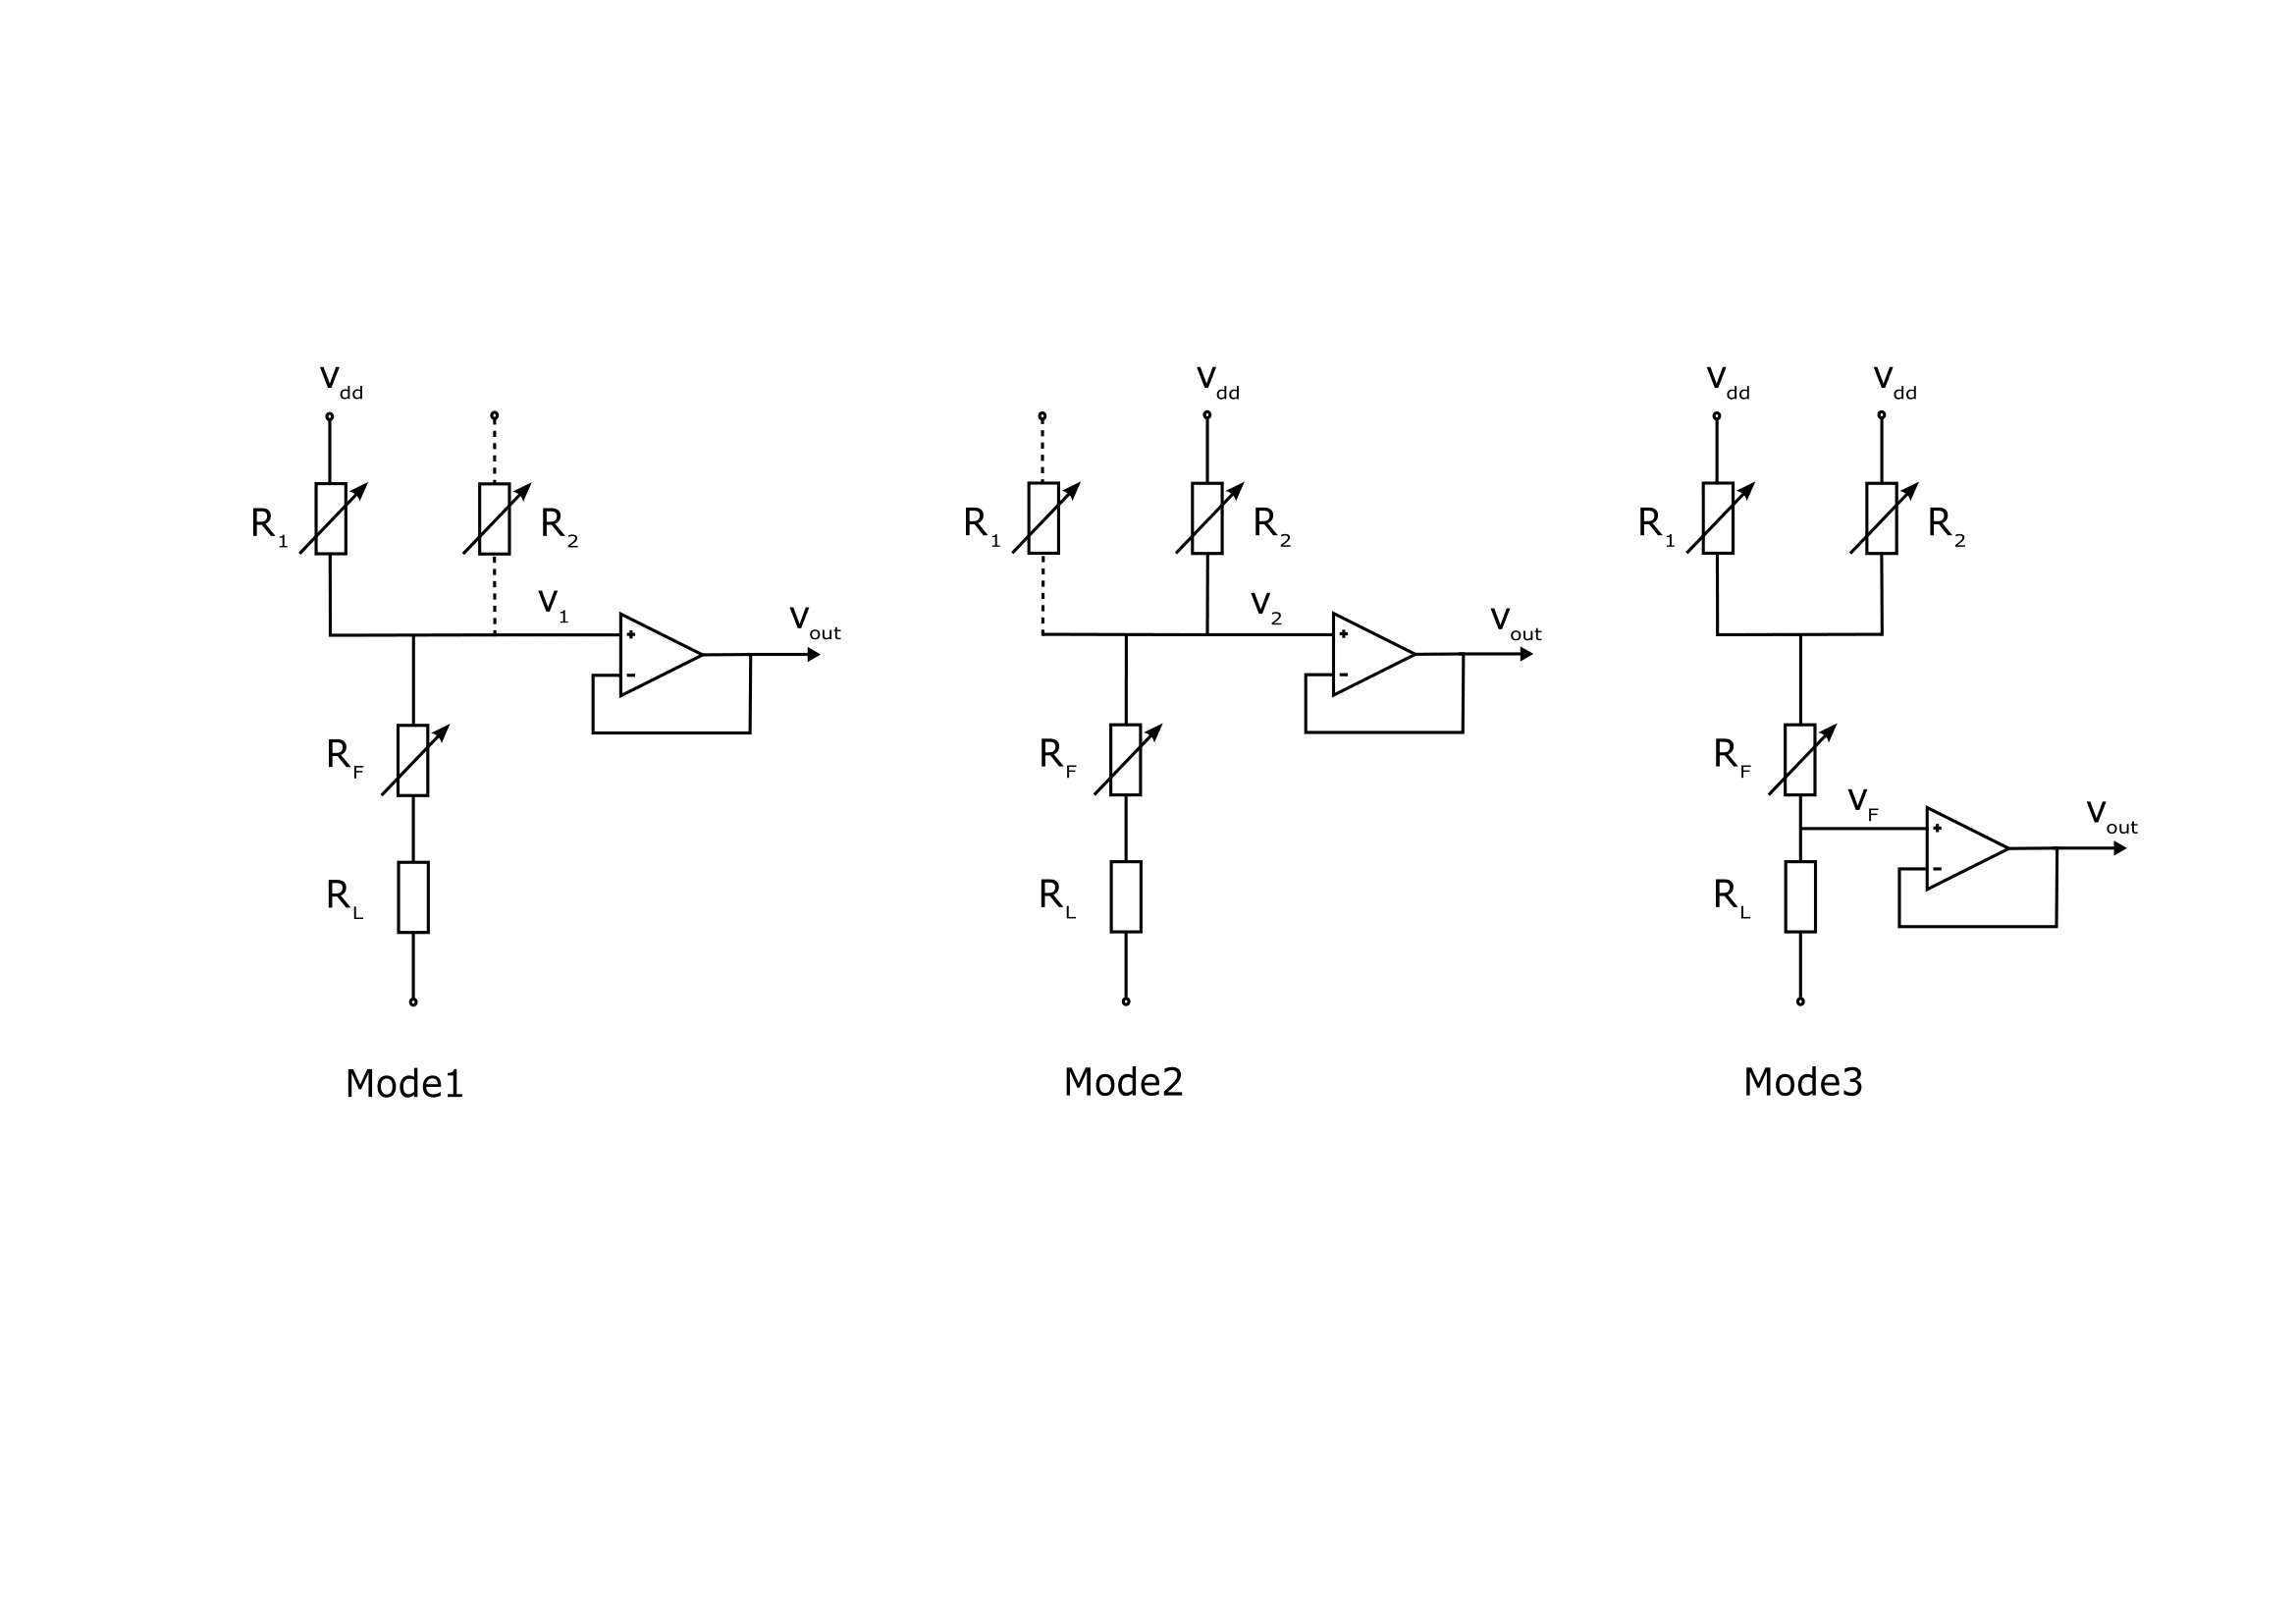
\includegraphics[width=\textwidth]{images./3MODES-1.png}
    \caption[Proposed system overview: System level]{3 operating modes}
    \label{fig:operatingmode}
\end{figure}  





\begin{equation}
    \frac{R_1(x)}{V_1(x)}=\frac{V_{dd}}{R_1(x)+R_r(F)+R_L}
    \label{eq:divider}
\end{equation}
leading to:
\begin{equation}
    R_1(x)=R_F(F)\cdot(\frac{V_{dd}}{V_1(x)}-1)
    \label{eq:r1}
\end{equation}
The same is valid for the second mode: 
\begin{equation}
    R_2(x)=R_F(F)\cdot(\frac{V_{dd}}{V_2(x)}-1)
    \label{eq:r2}
\end{equation}
For the third mode both Pin\textsubscript{1} and Pin\textsubscript{1} are set to logic high and the value of R\textsubscript{F} is measured. Also a voltage divider results in:
\begin{equation}
    \frac{V_F}{R_F(F)}=\frac{V_{DD}}{R_1(x)//R_2(x)+R_F(F)+R_L}
\end{equation}
\begin{equation}
    R_F(F)=\frac{R_1(x)\cdot R_2(x)}{(R_1(x)+R_2(x))}\cdot \frac{V_F}{V_{dd}-V_F}
    \label{eq:rf}
\end{equation}
Using equation \ref{eq:r1} and \ref{eq:r2}:
\begin{equation}
    R_F(F)=\frac{R_F^2(\frac{V_{dd}}{V_1}-1)(\frac{V_{dd}}{V_2}-1)}{R_F\cdot (\frac{V_{dd}}{V1}+\frac{V_{dd}}{V2}-2 )} \cdot \frac{V_F}{V_{dd}-V_F}
    \label{eq:underdtermined}
\end{equation}
Unfortunately \ref{eq:underdtermined} shows that the determinant of this system is zero, or in other words the system is non invertible. Therefore no unique solution for the system can be found. For the experiments in chapter \ref{ch:results} the load resistance is set a lot higher than the force depending resistor leading to accurate results even when ignoring the variation of R\textsubscript{F}.




\subsection{Switching modes}
Modern FSR have a typical rise time of no more than three microseconds  \cite{datasheet}. For a meaningful measurement each of the three modes has to be evaluated, resulting in force, area and position information. The microcontroller on a PSoC prototyping kit was programmed to transmit a sample and then switch to the next mode. Between each change of a mode there was a safety delay of 10ms introduced, still leading to a acceptable resolution while eliminating all possible rise time errors.




\subsection{Software}